\documentclass[fleqn]{article}
\usepackage[utf8]{inputenc}
\usepackage[margin=2.5cm]{geometry}
\usepackage{tikz}
\usepackage{xcolor}

\begin{document}
multinomial:\\
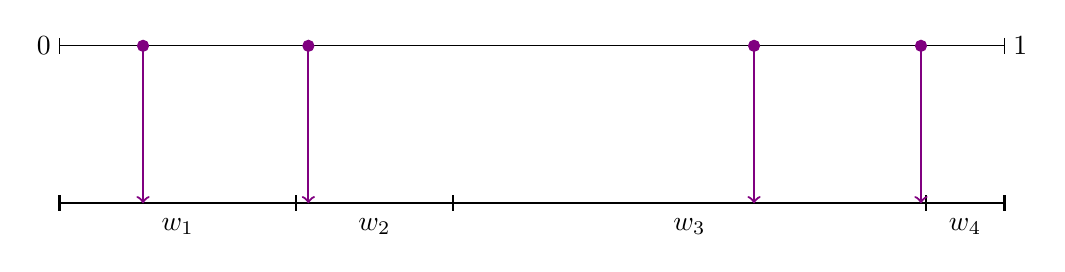
\begin{tikzpicture}
%parallel lines
\draw[thick] (0,0) -- (12,0);
\draw (0,2) -- (12,2);
% tick marks at ends
\draw[thick] (0,0.1) --(0,-0.1);
\draw[thick] (12,0.1) --(12,-0.1);
\draw (0,2.1) --(0,1.9);
\draw (12,2.1) --(12,1.9);
% tick marks indicating weights
\draw[thick] (3,0.1) --(3,-0.1);
\draw[thick] (5,0.1) --(5,-0.1);
\draw[thick] (11,0.1) --(11,-0.1);
% weight labels
\node at (1.5,-0.3) {$w_1$};
\node at (4,-0.3) {$w_2$};
\node at (8,-0.3) {$w_3$};
\node at (11.5,-0.3) {$w_4$};
% endpoint labels
\node at (-0.2,2) {$0$};
\node at (12.2,2) {$1$};
% uniform points
\filldraw[violet] (10.94,2) circle (2pt);
\filldraw[violet] (1.06,2) circle (2pt);
\filldraw[violet] (8.82,2) circle (2pt);
\filldraw[violet] (3.16,2) circle (2pt);
% arrows from random points
\draw[thick, violet, ->] (10.94,2) -- (10.94,0);
\draw[thick, violet, ->] (1.06,2) -- (1.06,0);
\draw[thick, violet, ->] (8.82,2) -- (8.82,0);
\draw[thick, violet, ->] (3.16,2) -- (3.16,0);
\end{tikzpicture}

stratified:\\
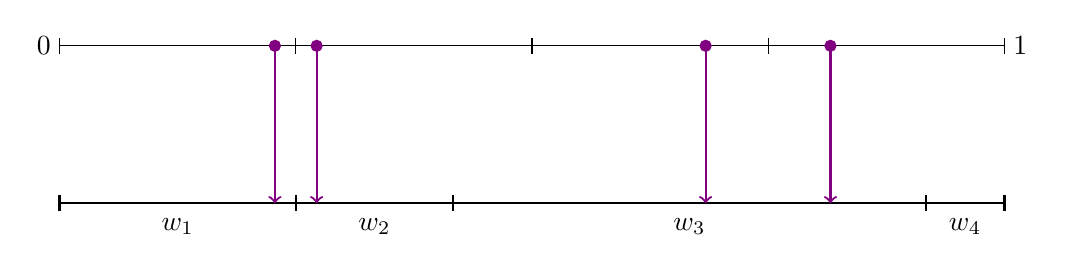
\begin{tikzpicture}
%parallel lines
\draw[thick] (0,0) -- (12,0);
\draw (0,2) -- (12,2);
% tick marks at ends
\draw[thick] (0,0.1) --(0,-0.1);
\draw[thick] (12,0.1) --(12,-0.1);
\draw (0,2.1) --(0,1.9);
\draw (12,2.1) --(12,1.9);
% tick marks indicating weights
\draw[thick] (3,0.1) --(3,-0.1);
\draw[thick] (5,0.1) --(5,-0.1);
\draw[thick] (11,0.1) --(11,-0.1);
% tick marks indicating sampling intervals:
\draw (3,2.1) --(3,1.9);
\draw (6,2.1) --(6,1.9);
\draw (9,2.1) --(9,1.9);
% weight labels
\node at (1.5,-0.3) {$w_1$};
\node at (4,-0.3) {$w_2$};
\node at (8,-0.3) {$w_3$};
\node at (11.5,-0.3) {$w_4$};
% endpoint labels
\node at (-0.2,2) {$0$};
\node at (12.2,2) {$1$};
% stratified points
\filldraw[violet] (2.735,2) circle (2pt);
\filldraw[violet] (3.265,2) circle (2pt);
\filldraw[violet] (8.205,2) circle (2pt);
\filldraw[violet] (9.79,2) circle (2pt);
% arrows from random points
\draw[thick, violet, ->] (2.735,2) -- (2.735,0);
\draw[thick, violet, ->] (3.265,2) -- (3.265,0);
\draw[thick, violet, ->] (8.205,2) -- (8.205,0);
\draw[thick, violet, ->] (9.79,2) -- (9.79,0);
\end{tikzpicture}

systematic:\\
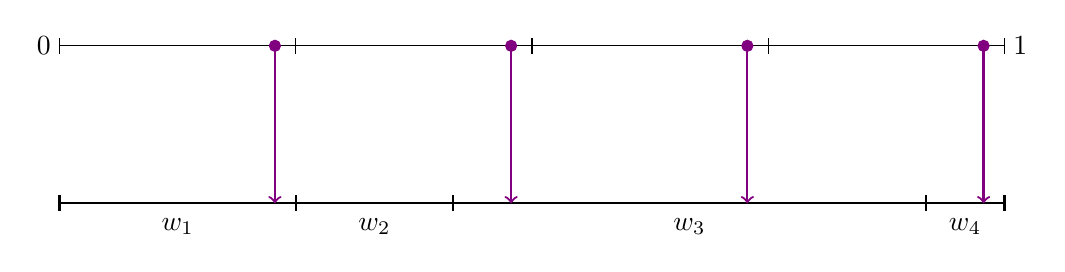
\begin{tikzpicture}
%parallel lines
\draw[thick] (0,0) -- (12,0);
\draw (0,2) -- (12,2);
% tick marks at ends
\draw[thick] (0,0.1) --(0,-0.1);
\draw[thick] (12,0.1) --(12,-0.1);
\draw (0,2.1) --(0,1.9);
\draw (12,2.1) --(12,1.9);
% tick marks indicating weights
\draw[thick] (3,0.1) --(3,-0.1);
\draw[thick] (5,0.1) --(5,-0.1);
\draw[thick] (11,0.1) --(11,-0.1);
% tick marks indicating sampling intervals:
\draw (3,2.1) --(3,1.9);
\draw (6,2.1) --(6,1.9);
\draw (9,2.1) --(9,1.9);
% weight labels
\node at (1.5,-0.3) {$w_1$};
\node at (4,-0.3) {$w_2$};
\node at (8,-0.3) {$w_3$};
\node at (11.5,-0.3) {$w_4$};
% endpoint labels
\node at (-0.2,2) {$0$};
\node at (12.2,2) {$1$};
% stratified points
\filldraw[violet] (2.735,2) circle (2pt);
\filldraw[violet] (5.735,2) circle (2pt);
\filldraw[violet] (8.735,2) circle (2pt);
\filldraw[violet] (11.735,2) circle (2pt);
% arrows from random points
\draw[thick, violet, ->] (2.735,2) -- (2.735,0);
\draw[thick, violet, ->] (5.735,2) -- (5.735,0);
\draw[thick, violet, ->] (8.735,2) -- (8.735,0);
\draw[thick, violet, ->] (11.735,2) -- (11.735,0);
\end{tikzpicture}
\end{document}